% !TEX root = ../Thesis.tex
%%
%%  Hochschule für Technik und Wirtschaft Berlin --  Projektabschlussbericht
%%
%% Kapitel 3 - Grundlagen
%%
%%

\chapter{Grundlagen} \label{Grundlagen}
\section{LoRa und LoRaWAN} \label{LoRa und LoRaWAN}

Der Begriff LoRa steht für \textbf{L}ong \textbf{R}ange und definiert dabei ein funkbasiertes Übertragungsverfahren auf der Bitübertragungs- (physical layer) und der Sicherungsschicht (MAC layer) im OSI-Schichtenmodell. Es wurde von der französischen Firma Cycleo, welche später von Semtech Corporation abgekauft wurde, entwickelt.

LoRa kann zu den sogenannten \textbf{L}ow-\textbf{P}ower-\textbf{W}ide-\textbf{A}rea-\textbf{N}etwork (LPWAN) Technologien zugeordnet werden, die einen energiesparsamen Betrieb und eine hohe Übertragunsreichweite aufweisen. Im Vergleich zu WLAN oder Mobilfunk, fällt jedoch die Daten- bzw. Bandbreite bei diesen Technologien relativ gering aus, sodass diese hauptsächlich bei drahtlosen Sensornetzwerken Anwendung finden, wo es darum geht Sensordaten mit einer geringen Datenrate über eine weite Funkstrecke zu übertragen. Ein Vergleich zu den funkbasierten Technologien (WLAN, LPWAN und Mobilfunk) stellt die Abb. \ref{fig:lpwan} dar.

\begin{figure}[h]
 \centering
 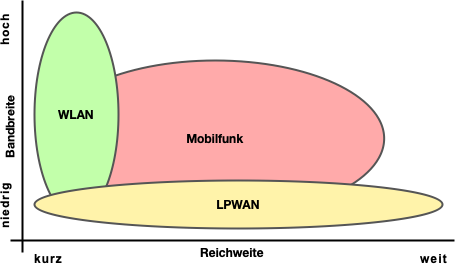
\includegraphics[width=0.7\textwidth]{pictures/lpwan-wlan-mobilfunk}
 \caption[Vergleich zwischen WLAN, Mobilfunk und LPWAN bezüglich der Bandbreite und Reichweite]{Vergleich zwischen WLAN, Mobilfunk und LPWAN bezüglich der Bandbreite und Reichweite \cite{lpwan2022}}
 \label{fig:lpwan}
\end{figure}

Die hohe Reichweite, bei gleichzeitig energiesparsamem Betrieb, erzielen die LPWAN Technologien mithilfe von Frequenzen unterhalb des 1 GHz Bereiches. Da LoRa ebenfalls zu den LPWAN Technologien zählt, nutzt diese in Europa die lizenfreien 433 und 868 MHz ISM-Frequenzbänder. Die Frequenzbänder unterscheiden sich jenach Land und Region auf der ganzen Welt. In den USA z.B. liegt der nutzbare Frequenzband bei 915 MHz. Das 433 MHz Frequenzband ist jedoch nur für unidirektionale Übertragung, wo man entweder nur Senden oder Empfangen kann, vorgesehen. Hingegen ist das 868 MHz Band bidirektional, das heißt, dass damit das gleichzeitige Senden und Empfangen gewährleistet ist \cite{lpwan2022}. 

Die jeweiligen Frequenzbänder haben eine bestimmte Frequenzbandbreite und werden wiederum in sogenannte Funkkanäle unterteilt, mit einer bestimmten Kanalbandbreite, um das gegenseitige stören gleicher Frequenzen zu minimieren. So weist z.B. das 868 MHz Frequenzband eine Frequenzbandbreite zwischen 863 und 870 MHz auf \cite{Staniec2020}. So können benachbarte Funkknoten, die sich im gleichen 868 MHz Frequenzband befinden, aber einen unterschiedlichen Funkkanal nutzen, gleichzeitig senden und empfangen, ohne sich dabei zu stören. 

Darüberhinaus werden weitere regulatorische Maßnahmen ergriffen, wie die Festlegung einer Zeit in Form eines \textbf{D}uty-\textbf{C}ycles (DC), welches angibt, wie lange ein Funkknoten auf das Medium pro Tag zugreifen darf. Dieser ist ein prozentualer Wert und liegt bei LoRa normalerweise bei 1\% oder 10\% je nach Funkkanal und Sendeleistung \cite{Staniec2020}. 

Die Abbildung \ref{fig:868-band} zeigt das 868 MHz-Frequenzband mit den jeweiligen Funkkanälen, deren Bandbreite (in kHz), der äquivalenten Strahlungsleistung (in dBm) und des jeweiligen Duty Cycles an . 

\begin{figure}[h]
 \centering
 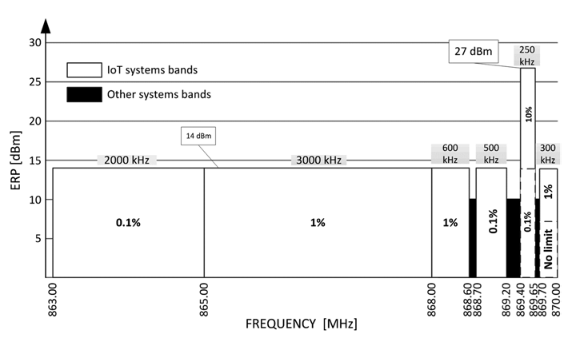
\includegraphics[width=0.9\textwidth]{pictures/868-band}
 \caption[Aufteilung des 868-ISM-Bandes in Funkkanäle nach ETSI EN 300 220-2]{ \cite{Staniec2020}}
 \label{fig:868-band}
\end{figure}

Weitere Möglichkeiten zur Verhinderung der gegenseitigen Störung sind die definierten Zugriffsverfahren auf das Medium, die bei LPWAN auch als \textbf{P}olite-\textbf{M}edium-\textbf{A}ccess (PMA) heißen. Darunter zählt das sogenannte \textbf{C}lear-\textbf{C}hannel-\textbf{A}ssessment (CCA), welches wiederum in \textbf{A}daptive-\textbf{F}requency-\textbf{A}gility (AFA) und \textbf{L}isten-\textbf{B}efore-\textbf{T}alk (LBT) eingeteilt werden kann. Dabei ähnelt das CCA-Zugriffsverfahren sehr stark dem Carrier-Sense-Multiple-Access/Collision-Avoidance (CSMA/CA) Zugriffsverfahren bei z.B. WLAN.

Bei dem AFA Verfahren, wird einerseits die Datenrate hinsichtlich der Kanaleigenschaften angespasst und andererseits ein geeigneter Funkkanal mittels spezieller Algorithmen, die die optimale Lastverteilung zwischen den jeweiligen Funkkanälen berechnen, ausgewählt. Das LBT Verfahren stellt sicher, dass immer nur ein Funkgerät auf einen Funkkanal zugreifen kann, um die gegenseitige Störung zu verhindern. So „lauscht“ (listen) es auf den Funkkanal auf dem es zugreifen möchte zunächst einmal, um festzustellen, ob es frei ist, bevor es darauf zu „sprechen“ (talk) beginnt. Wenn das Funkgerät merkt, dass der Kanal momentan besetzt ist, dann wartet es eine gewisse Zeit, die normalerweise zwischen 5 und 10ms beträgt, ab, bevor es nochmal versucht auf den Kanal zuzugreifen \cite{Staniec2020}. 

Die Reichweite von LoRa beträgt zwischen 2-5 km in urbanen und 5-15 km in ländlichen Regionen mit keiner direkten Sichtverbindung (non-line-of-sight). Wenn es eine direkte Sichtverbindung (line-of-sight) zwischen den Funkmasten gibt, dann kann die Reichweite auch weit über 15 km erreichen. Die Datenrate liegt dabei im Bereich zwischen 0.3-5.5 kBit/s und die maximale Übertragungsleistung bei 25 mW \cite{lora2022}. Der aktuelle Rekord, bei dem die Sensorwerte noch empfangen konnten, liegt bei einer unglaublichen Reichweite von 766 km, welcher im Juli 2019 aufgestellt wurde\footnote{https://tech-journal.semtech.com/university-of-zaragoza-breaks-long-range-lorawan-based-signal-record}.

Die hohe Reichweite bei gleichzeitig geringem Energieverbrauch ist abgesehen von der niedrigen Frequenz, der speziellen Modulations- bzw. Übertragungsverfahren zu verdanken. LoRa benutzt die sogenannte \textit{Chirp-Spread-Spectrum} (CSS) Modulationstechnik, bei der sich die Frequenz eines Signals (0 oder 1) innerhalb eines definierten Frequenzbereiches gleichmäßig ändert (siehe Abb. \ref{fig:css}). 

\begin{figure}[h]
 \centering
 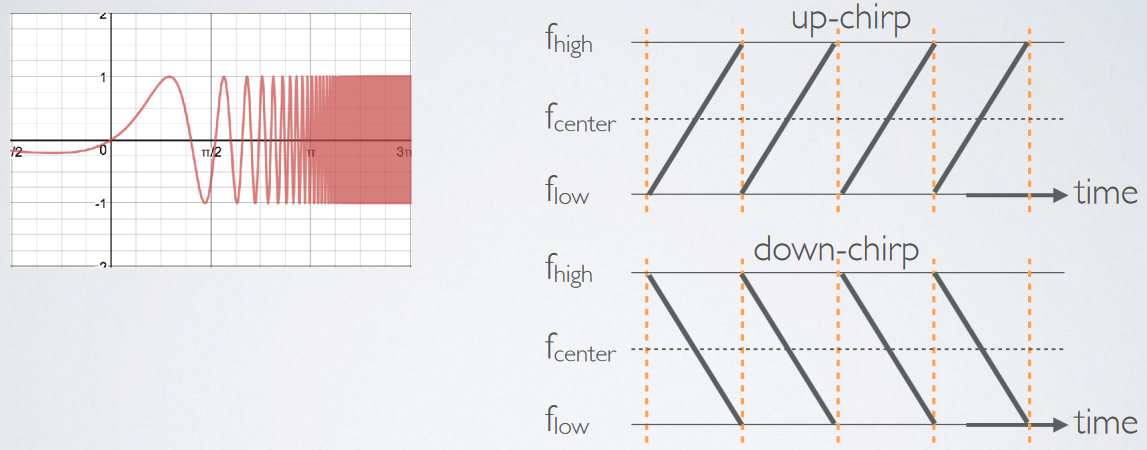
\includegraphics[width=0.7\textwidth]{pictures/chirp-sf}
 \caption[chirp spread spectrum]{chirp spread spectrum \cite{lora2020}}
 \label{fig:css}
\end{figure}

Die gleichmäßige Änderung der Frequenz innerhalb eines definierten Frequenzbereiches wird als chirp (zwitschern oder zirpen) bezeichnet und ist in der Natur weit verbreitet. So kommunizieren z.B. Vögel oder Delphine ebenfalls über die zeitliche Änderung der Frequenz. Dies hat den Vorteil, dass äußere Störungen einen geringeren Einfluss auf die Signalqualität ausüben und somit das Signal-Rausch-Verhältnis sich verbessert.    


 


\section{MQTT} \label{MQTT}

\ldots


